% https://texample.net/tikz/examples/yin-and-yang/

% Yin and yang
% Author: Thomas G. Kristensen
\documentclass{article}

\usepackage{tikz}
\begin{document}

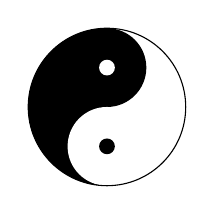
\begin{tikzpicture}

  %color one half of a unit circle
  \begin{scope}
    \clip (0,0) circle (1cm);
    \fill[black] (0cm,1cm) rectangle (-1cm, -1cm);
  \end{scope}

  %fill heads
  \fill[black] (0,0.5) circle (0.5cm);
  \fill[white] (0,-0.5) circle (0.5cm);

  %fill eyes
  \fill[white] (0,0.5) circle (0.1cm);
  \fill[black] (0,-0.5) circle (0.1cm);

  %outer line
  \draw (0,0) circle (1cm);

\end{tikzpicture}

%%% An alternative method suggested by Robert Papanicola
%%% There are unfortunately some visual artifacts due to
%%% the
%%\begin{tikzpicture}
%%%\fill[black, rounded corners=1cm] (0,-1) -- (-1,-1) -- (-1,1) -- (0,1) {
%%%     [rounded corners=0.5cm]-- (0.5,1) -- (0.5,0) -- (0,0) -- (-0.5,0)
%%%     -- (-0.5,-1) -- (0,-1)} ;
%%\fill[black, rounded corners=0.5cm] (0,-1) -- (-1,-1) -- (-1,1) -- (0,1) {
%%     [rounded corners=0.5cm]-- (0.5,1) -- (0.5,0) -- (0,0) -- (-0.5,0)
%%     -- (-0.5,-1) -- (0,-1)} ;
%%\draw (0,0) circle (1cm);
%%\draw[fill=white] (0,0.5) circle (0.1cm);
%%\draw[fill=black] (0,-0.5) circle (0.1cm);
%%\end{tikzpicture}

\end{document}
